\documentclass[a4paper,10pt]{article}

\usepackage{ifpdf}
\ifpdf
  \usepackage[pdftex]{graphicx}
  \graphicspath{{images/}}
\else
  \RequirePackage[dvipdfm, CJKbookmarks, bookmarks=true, bookmarksnumbered=true%
                unicode,%
             colorlinks,%
         citecolor=blue,%
             hyperindex,%
       plainpages=false,%
      pdfstartview=FitH]{hyperref}
  \AtBeginDvi{\special{pdf:tounicode UTF8-UCS2}}
  \usepackage[dvipdfm]{graphicx}
  \graphicspath{{images/}}
  \DeclareGraphicsExtensions{.eps}
\fi

%\RequirePackage{CJKutf8,CJKnumb,CJKulem}
\RequirePackage{CJKutf8,CJKnumb}
\RequirePackage{color,verbatim,cite}
\RequirePackage{texnames,makeidx,indentfirst}
\RequirePackage{amsmath,amssymb,amsfonts,bm,manfnt}
\RequirePackage{fancyhdr,titlesec,datetime}
\RequirePackage{wasysym,longtable,multirow,bigstrut}
\usepackage[section]{placeins}
\usepackage[left=2.54cm,right=2.54cm,top=3.3cm,bottom=2.6cm]{geometry}
\usepackage[caption=false,font=footnotesize]{subfig}

\AtBeginDocument{\begin{CJK*}{UTF8}{song}\CJKtilde\CJKindent\CJKcaption{utf8}}
\AtEndDocument{\end{CJK*}}

\setlength{\parskip}{0.75ex plus .2ex minus .5ex}
\renewcommand{\baselinestretch}{1.2}

\hypersetup {
    pdftitle={无线传感器网络中的位置相关安全},
    pdfauthor={杨文博}
}

\title{无线传感器网络中的位置相关安全}
\author{杨文博}

\begin{document}

\maketitle

\section{项目的立项依据} 

(研究意义、国内外研究现状及发展动态分析,需结合科学研究发展趋势来论述科学意义;或结合国民经济和社会发展中迫切需要解决的关键科技问题来论述其应用前景。附主要参考文献目录)

上世纪末到本世纪初,通信、嵌入式和分布式计算技术有了飞速的发展,同时得益于微机电系统的长足进步,人们研制出各种不同功用的廉价微型传感器。这些传感器可以感知、测量并收集所处的环境信息,经过通信网络传输给传感器的部署者。无线传感器网络就是由大量支持无线通信的廉价传感器节点组成的分布式、自组织的无线网络。它可以广泛使用在国防军事、国家安全、环境检测、火灾预警、仓储物流、交通管理、医疗卫生和灾难救援等许多领域,帮助人们及时获得有价值的目标环境信息,协助管理者做出正确的决策。

无线传感器节点一般情况下由感应模块、处理器、内存、能量供应、无线模块和控制单元组成。装配着不同的感应模块的传感器可以感知和测量物理环境的不同信息,例如湿度、温度、压力、震动、风速、声音、辐射、有毒气体含量等等,因而可以应用于不同的环境中。由于其廉价性和微型化,无线传感器所采用的处理器一般比较低端,不支持如浮点运算、多媒体指令等一些高级功能。它们一般都只配备少量的内存,所收集到的信息将使用无线方式传输到基站。一般情况下,无线传感器节点的能量主要由电池供应,根据环境的不同可以采用太阳能等其它的能量供应方式作为后备能源。

典型的无线传感器网络一般由数十到数千个无线传感器节点组成,由人工或者机械撒播在目标区域,用来监测目标区域内的特定环境信息。受无线传感器节点体积小、数量大、资源受限的限制,无线传感器网络往往具有以下特点:

\begin{enumerate}

\item 通信的带宽、稳定性和安全性较差。由于采用无线信号通信,受信道本身物理特性的限制,无线传感器网络的通信质量和稳定性往往较差;考虑到无线信号的开放性,其更容易受到信道窃听、伪装、拒绝服务等攻击,需要考虑一些特别安全需求。

\item 网络资源受限。无线传感器节点往往不具有长期的电源供应,节点设计的计算能力、存储空间都要比一般的有线网络节点要小得多。在设计网络网络结构时需要特别考虑到能耗因素,避免部分节点能源耗尽导致整个网络失灵。

\item 树形路由、多跳转发。基站是收集信息的汇聚点,所以无线传感器网络一般构成以基站为根节点的树形结构;由于节点天线发射功率小,信号的覆盖范围受限,无线传感器节点间通信往往需要经过多跳转发,其转发由传感器节点完成,没有专门的路由设备。

\end{enumerate}

由于受到上述特点的限制,无线传感器网络的组网、路由、数据传输的稳定性和安全性在设计时都需要特别考虑。

虽然面临着许多困难,但是由于其广泛的应用前景,无线传感器网络在工业应用和技术研发方面保持着非常强劲的增长势头。专注于无线技术的市场调研公司~ON World~在~2007~年~9~月发布的报告《无线传感器网络产业》中预计到~2011~年,世界市场无线传感器网络系统与服务价值将升至约~46亿~美元,比~07~年增长~5~亿美元~\footnote{ON World Research: \href{http://onworld.com/smartindustries/}{WSN for Smart Industries - A Market Dynamics Report }};市场研究机构~WTRS (West Technology
Research Solutions)~在~2008~年~12~月发布的《无线传感器网络技术趋势报告》中预测可用于无线传感器网络的低功耗~WiFi~芯片市场将在~2008~到~2013~年间保持~322\%~的复合年均增长率~\footnote{WTRS: \href{http://www.wtrs.net/wcntechtrends.htm}{Wireless Sensor Network Technology Trends Q4 2008}};ON World~公司~2009~年~1~月发布的《无线传感器网络研发趋势》报告预测到~2012~年,全球无线传感器网络研发支出将达到~13~亿美元,是~2007~年研发支出的~2.5~倍~\footnote{ON World Research: \href{http://onworld.com/wsn/}{Wireless Sensor Networks — R\&D Trends and Funding Opportunities }}。

我们可以看到,对无线传感器网络的研究,不仅是科技发展战略上的需求,而且在工业应用和服务上也有非常广大的发展前途。由于无线传感器网络往往用于监控敏感信息,或者部署在危险或者充满敌意的环境中,无线传感器网络的安全通常会受到严重的威胁。因此对其安全技术的研究是无线传感器网络研究中非常重要的一环,没有保证网络安全的技术,就不可能有可用的无线传感器网络。

位置信息是无线传感器网络中的一项重要信息。比如在环境监测的应用中,监测程序根据传感器所收集到的环境信息,检测是否有事件发生。在某事件发生时,管理者往往需要知道该事件发生的位置以及感知该事件的传感器节点的位置。没有位置信息的事件报告是不完整的,也是没有用处的。无线传感器节点的位置信息有着非常广泛的应用,包括数据的识别和关联、节点定位、对指定区域节点的管理和查询、评估节点密度和覆盖范围、网络能量分布图、基于地理位置的路由、目标追踪等。因此,保证节点正确、安全地获得和使用位置信息,对无线传感器网络的应用有着非常重要的作用。

虽然对无线传感器网络定位技术的研究起步较早,但无线传感器网络安全定位技术却是一个相对较新的研究课题,对其系统的研究起源于~2003~年左右。目前来讲,无线传感器网络的安全定位技术按照其算法和实现方式可以大致分为用密码学手段、异常行为检测和屏蔽、攻击容忍的鲁棒位置算法和位置验证技术等几大类~\cite{Boukerche2008},如图~\ref{wsn_sec_pos}~所示。下面我们对这几大类技术进行一些简单的说明和分析。

\if false
\begin{figure}[htbp]
  \centering
  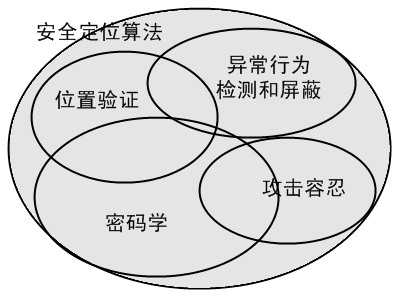
\includegraphics[width=.9\textwidth,keepaspectratio]{wsn_sec_pos}
  \caption{\label{wsn_sec_pos}~WSN~安全定位算法}
\end{figure}
\fi

\begin{itemize}

\item 密码学手段(Security through Cryptography)。密码学是保证信息安全的重要工具之一,因此也被广泛用于保护定位系统传输数据的安全中。数据包加密和数据源认证是安全定位系统中被广泛采用的密码学手段。

L. Lazos~和~R. Proovendran~等人提出的~SeRLoc \cite{Lazos2005}、~HiRLoc \cite{Lazos2005a}~和~ROPE \cite{Lazos2006},S. \v{C}apkun~和~J.P. Hubaux~提出的~SPINE \cite{Capkun2006}~等方案,都采用了加密和数据源认证方法来保证~beacon~消息的安全传输。SeRLoc~采用全局的密钥来加密定位者消息,用私密口令的哈希值链实现对定位者消息的数据源认证~\cite{Lazos2005};SPINE~中提出了可验证的多向法(Verifiable Multilateration),第一次将距离边界协议(Distance Bounding Protocol)引入无线传感器网络位置验证中,在可验证的多向法中至少三个验证节点独立使用带加密的距离边界协议计算某节点的位置,并将计算得的距离上传到一个~CA(Central Authority)~,CA~使用最小均方误差(Minimum Mean Square Error, MMSE)或者其它方法来计算并验证节点位置是否在误差范围和扇区相交区域内~\cite{Capkun2006};HiLoc~是在~SeRLoc~的基础上,利用可旋转和可变发射功率的定向天线来达到高精度定位的目的。它与~SeRLoc~相同,也使用全局的密钥来加密定位者消息,用私密口令的哈希值链实现对定位者消息的数据源认证~\cite{Lazos2005a};ROPE~方案在~SeRLoc~基础上增加了距离边界协议,但是~ROPE~的计算和验证过程和~SPINE~不同,不需要~CA~的参与~\cite{Lazos2006}。

\item 异常行为检测和屏蔽(Misbehavior Detection and Block)。防范对无线传感器网络定位系统的攻击还可以使用检测恶意节点的异常行为并屏蔽该恶意节点的方法。此方法主要用来防范对定位算法中位置计算部分的攻击。D. Liu~等在~\cite{Liu2005c}~提出了两个检测恶意定位者节点的方法:一个是节点用其与目标节点的坐标距离和实测距离(由信号估计得来)相比较,如果误差大于某个阈值,就认为该目标节点传输了虚假的坐标值,视其为恶意节点;另一个是节点用其与目标节点的通信往返时间与正常往返时间比较,如果误差大于某个阈值,则认为该目标节点进行了重放攻击,视其为恶意节点。A. Srinivasan~等在~\cite{Srinivasan2006}~中提出了一个分布式的基于信誉的定位者节点信任系统(Distributed Reputation-based Beacon Trust System, DRBTS)。每个定位者节点维护一个邻居定位者节点的信誉表(Neighbor-Reputation-Table, NRT),节点间交换~NRT~,使用基于投票的方式选择可信节点组。

\item 攻击容忍的鲁棒位置算法(Robust Position Computation)。解决恶意节点问题的另一种办法是接受恶意节点存在这一现实,使用鲁棒的位置计算方法来消除恶意信息的影响。研究者一般假设正常节点多于恶意节点,然后使用统计学方法来消除恶意节点影响。

D. Liu~等在~\cite{Liu2005b, Liu2008a}~中提出了实现攻击容忍的两个实现。一是利用最小均方误差估计(Minimum Mean Square Estimation, MMSE)来识别并排除恶意节点。节点使用接收到的定位信息集合的不同子集计算均方误差,最后选取均方误差满足可接受阈值的最大子集作为一致性定位信息集合,计算自身位置,可使用贪心算法减少其计算量;第二个方案基于投票机制。节点可能出现的位置区域被量化成网格,节点利用收到的定位信息对其可能位置进行投票,得票最多的网格区域中央被选为该节点所在位置。Z. Li~等在~\cite{Li2005a}~中提出了使用最小均方算法(Least Mean Squares, LMS)代替最小二乘法(Least Squares)来容忍对定位算法的攻击;S. Misra~等在~\cite{Misra2007}~中提出了使用基于聚类的方法来容忍恶意的定位者信息,使用通用合并方法对定位者信息的交点集做聚类,选择最大的聚类作为可信定位者信息交点集,然后再使用最小均方误差算法来计算节点位置。

S. Zhong~等在~\cite{Zhong2008}~中证明了:在使用定位者节点提供定位参考信息的无线传感器网络中,假设~$n$~为节点~A~周围的定位者节点数,当其中的恶意节点超过~$\frac{n-2}{2}$~时,不存在算法能保证节点~A~的定位精度;当恶意节点不大于~$\frac{n-3}{2}$~时,存在算法可以保证节点~A~有一定的定位精度,~\cite{Zhong2008}~中还给出了两种满足该条件的示例算法。

\item 位置验证技术(Location Verification)。位置验证也是安全定位研究中非常重要的一个方面,它将视角从直接解决安全定位问题转向验证定位结果是否正确。我们前文中提到的一些方案,比如~SPINE \cite{Lazos2005a}, ROPE \cite{Lazos2006}~和~HiLoc \cite{Lazos2005a}~,也在安全位置计算过程中加入了位置验证过程。

N. Sastry~等在~\cite{Sastry2003}~中首先提出安全位置验证(Secure Location Verification)的概念,并给出了一个使用无线射频和超声波测距的距离边界协议~Echo~方案。W. Du~等提出了一个在定位过程结束后,检测位置异常的节点~LAD(Localization Anomaly Detection)~\cite{Du2006}~方案。此方案中,节点被分组部署,因而可预知可能的周围节点信息,根据部署信息和定位结果,若某节点的声称位置与其所属组节点的位置差距过大,则认为该节点位置异常。S. \v{C}apkun~等提出利用可信的隐藏和移动基站来对节点的位置进行验证的方案~\cite{Capkun2006a, Capkun2008}。由于部分基站位置隐藏(无线电静默)或者移动,攻击者无法预知该类基站位置,该类基站通过监听信道可以获得更真实的数据,判断节点是否处于声称的位置。

\end{itemize}

除了安全定位技术以外,在某些环境中,我们还关心如何保护传感器节点位置信息不会泄露出去。M. Gruteser~等在~\cite{Gruteser2003}~中首先提出使用数据隐藏(降低数据精度)、分层数据融合和加密通信的方法保证位置信息的私密性;C. Ozturk, Y. Zhang~和~W. Trappe~提出了利用抵抗流量分析的手段来防止敌手通过追踪通信得到节点位置,主要使用随机路由和增加虚假流量的方式~\cite{Ozturk2004},这些方式的主要问题是为了达到匿名性引入不必要的通信,因而使得能量消耗过大~\cite{Xiao2006};Y. Xi~等对~C. Ozturk~的方法进行了改进,提出了使用双向贪心随机游走的~GROW(Greedy Random Walk)~方案~\cite{Xi2006},~GROW~要求消息的发送者和接收者都进行若干跳的随机游走,当发送者和接收者的随机游走路径发生交叉时,就用该路径进行消息的传输。

\section{项目的研究内容、研究目标,以及拟解决的关键科学问题} 

由于无线传感器网络往往由廉价、微型的节点组成,节点的计算能力、能源供应和发射功率受到很大限制。为了降低能耗和保证网络的可用性,我们应当研究更简单和鲁棒的安全定位算法。

现阶段提出的安全定位方法中,有一部分需要部分节点配备特殊的硬件支持才能实现安全定位。比如~SeRLoc \cite{Lazos2005}~中定位者节点必须配备定向天线,HiRLoc \cite{Lazos2005a}~中假设定位者节点具有可旋转的定向天线,\cite{Capkun2006a, Capkun2008}~中要求隐藏基站有普通节点不可发觉的秘密信道,或者移动基站具有可高速移动的能力,SPINE \cite{Capkun2006}~和~ROPE \cite{Lazos2006}~等要求节点的时钟精确到纳秒级。此类算法对传感器节点硬件的要求在目前的技术水平上很难达到,特别是在廉价、微型、低功耗的限制下。将这些算法应用到当前的无线传感器设备上时,算法要么完全无法工作,要么定位精度达不到要求。

能够在当前的无线传感器节点上部署的安全定位算法中,大部分使用统计学方法和异常检测方法来降低或者消除恶意定位信息对最终定位结果的影响。但是目前使用的统计学方法往往需要根据不同的信息集对定位结果或误差进行多次计算和比较,特别是在精度要求较高时,计算开销非常大。异常检测方法需要借助于精确的距离估计,在距离估计受到环境干扰或者是恶意节点的蓄意破坏时,容易发生虚警和漏警。

孤立地考虑安全定位算法,将安全定位算法与其它安全措施独立实现在传感器的系统中,当算法之间有相似之处时,比如加解密模块,将会造成比较大的存储空间和能源浪费。设计能与其它安全方案相结合的安全定位算法,算法间共享相同的模块和接口,也许是降低内存需求和能量消耗的一种很有效的方法。

因此,我们希望能设计出一种更简单和鲁棒,并且能与其它安全算法相结合的安全定位算法。该算法能够适用于当前无线传感器设备之上,能容忍恶意节点的攻击,具有更低的能量消耗,为相关服务提供更可靠的位置信息。

\section{拟采取的研究方案及可行性分析} 

(包括有关方法、技术路线、实验手段、关键技术等说明)

综合评估现有安全定位方法的特点与不足。从抵御的攻击类型、硬件要求、定位精确度、算法复杂度、通信开销、可扩展性等几个方面对它们进行分类比较,寻找现有方案的优点和特性,挖掘仍然存在的漏洞和不足。

对基于统计和异常检测的定位算法进行详细研究,分析定位算法背后的统计模型,探索每个模型适用的范围以及对错误数据的容忍程度,寻找其它可适用于无线传感器网络定位算法的更健壮的统计模型,并使用模拟和仿真等手段与已有算法相比较。

比较安全定位与其它安全方案,分析可共同利用的信息和模块。研究安全定位与密钥管理、数据融合、安全路由等其它安全方案所需的信息和算法模块组成,从密码算法、协议内容等处寻找可供共同利用的模块或信息,综合考虑多种安全方案,以达到优化算法或协议,减少计算量和通信量的目的。

提出新的安全定位方案并进行仿真实验。以提高定位算法的安全性和健壮性、降低算法和协议的复杂度为目的,构造新的安全定位算法,或者与其它安全方案结合,设计安全定位方案。分析安全定位方案面临的攻击类型和抵抗攻击的能力,进行仿真实验并与已有方案进行比较,评估安全方案的有效性和可行性。

\section{本项目的特色与创新之处} 

\begin{enumerate}
\item 采用新的安全定位方法,提高定位算法的安全性和健壮性。
\item 分析多种安全方案的可结合之处,共同协作减少复杂度。
\item 考虑位置信息的不同安全应用,简化整体安全方案。
\end{enumerate}

\bibliographystyle{IEEEtran}
\bibliography{IEEEfull,wsn}

\end{document}

